In this section we review the basic definitions and terms related to the domain
of frontier-based exploration, as well as a formal definition of the
frontier-based exploration problem (Section~\ref{section:definitions}). We briefly discuss
common state-of-the-art techniques for performing a Simultaneous
Localization and Mapping (Section~\ref{section:slam}), which underly existing
approaches to exploration. We then present the \WFD algorithm
which searches for frontiers on the map (Section~\ref{section:wfd}).

\subsection{Frontier-Based Exploration: Definitions}
\label{section:definitions}
In this section we define and explain the terms that are used in the following
sections. We assume the robot in question uses an occupancy-grid map
representation in the exploration process (Figure \ref{fig:frontiers}) within the map:

\noindent{\bf Unknown Region} is a territory that has not been covered yet by
the robot's sensors.
	
\noindent{\bf Known Region} is a territory that has already been covered by the
robot's sensors.
	
\noindent{\bf Open-Space} is a \emph{known region} which does not contain an
obstacle.

\noindent{\bf Occupied-Space} is a \emph{known region} which contains an
obstacle.

\noindent{\bf Occupancy Grid} is a grid representation of the environment. Each
cell holds a probability that represents if it is occupied.

\noindent{\bf Frontier} is the segment that separates known (explored) regions
from unknown regions. Formally, a frontier is a set of \emph{unknown} points that each have at
least one \emph{open-space} neighbor.

\begin{definition}
Suppose we are given a temporal sequence of observations $\langle
O_0,\ldots,O_t\rangle$ (time 0 to time $t$), where each observation $O_x$ is a
tuple $\langle G_x, P_x, R_x\rangle$ composed of: (i) the occupancy-grid $G_x$
of time $x$; (ii) the robot pose $P_x$ (in occupancy-grid coordinates); and
(iii) the range sensor readings $R_x$ originating at the robot location (given
in either ego-centric polar coordinates, or in occupancy-grid coordinates).
The \emph{Frontier Detection Problem} is to return all frontiers existing at
time $t$, given the sequence.
\end{definition}


% \begin{figure}
%  \centering
%  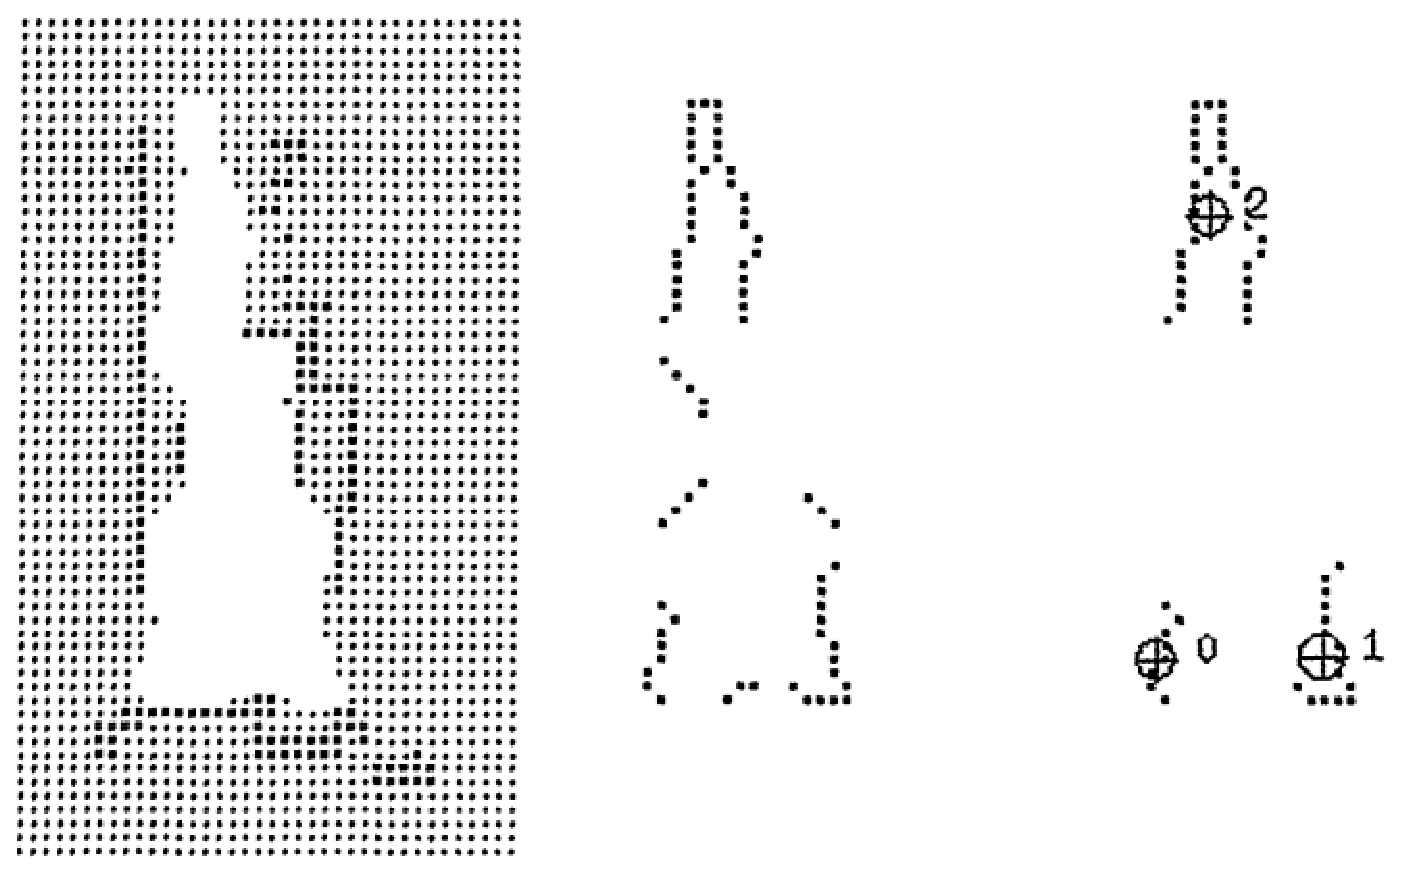
\includegraphics[width=0.8\columnwidth,keepaspectratio]{frontiers_example}
%  \caption{Evidence grid, frontier points, extraction of different frontiers (from left to
%  right). Taken from \protect\cite{yamauchi_frontier-based_1998}.}
%  \label{fig:frontiers}
% \end{figure}

\begin{figure}
 \centering
 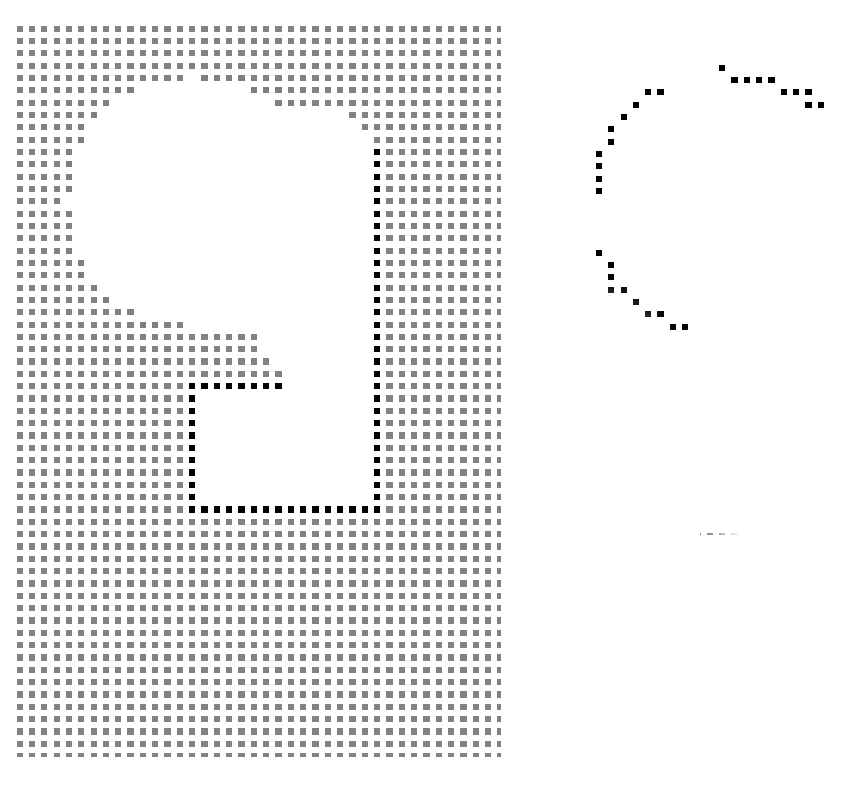
\includegraphics[width=0.5\columnwidth,keepaspectratio]{octave/frontiers_combined_fixed}
 \caption{Evidence grid, frontier points (from left to
 right).}
 \label{fig:frontiers}
\end{figure}

Existing algorithms for frontier detection rely on edge-detection methods. The
algorithms systematically search for frontiers all over the occupancy-grid,
i.e., both in known and unknown regions.

\subsection{Simultaneous Localization and Mapping Methods}
\label{section:slam}
Simultaneous Localization and Mapping (\emph{SLAM}) is a method utilized by
autonomous mobile robots for building a map of an unknown environment while at
the same time navigating the environment using the map. The term \emph{SLAM} was
originally developed by Leonard et al. \cite{leonard1991mobile,durrant2006simultaneous}.
In \emph{SLAM} both the trajectory of the mobile robot,
its location and the location of the landmarks observed by the robot are
estimated without using any \emph{a priori} knowledge of the environment.
\emph{SLAM} is a concept and hence, there are various algorithms in literature
which deal with the \emph{SLAM} problem:  

\paragraph{Extended Kalman Filter}
The \emph{Kalman Filter} (\emph{KF}) is a method for implementing Bayes
filters.
It was invented by Rudolph Emil Kalman \cite{welch1995introduction,
Thrun2005Probablistic} to apply filtering and perform prediction in linear
systems. In Kalman Filter, beliefs are represented by moments (i.e., by the mean
and the covariance). Markov assumptions are held and the posteriors are
Gaussian. Kalman filters are based on \emph{linear} system dynamics. However,
real-world systems are seldom linear in practice (e.g., robot which moves in a
cyclic path). The \emph{Extended Kalman Filter} (\emph{EKF}) uses a non-linear
functions that describe the system dynamics. In \emph{EKF-SLAM} systems, there
is only one map (part of the system state) that is composed from the observed
landmarks.
  
\paragraph{Particle Filter}
A \emph{Particle Filter} (also known as \emph{sequential Monte Carlo method}) is
a model estimation method which is based on simulation. Particle Filter is the
online version of \emph{Markov chain Monte Carlo} (\emph{MCMC}) methods
\cite{HASTINGS01041970,geyer1992practical,neal1993probabilistic}.
With sufficient samples, a particle filter is often an alternative to \emph{EKF}
with the advantage that it approaches the Bayesian optimal estimate and so it
is more accurate than \emph{EKF}. Each particle is a possible hypothesis of what
is the true world state at a certain time, that is, each particle is an
instance of the system state at a certain time. By state we refer to a
collection of variables such as the map of the explored environment, the robot
position etc. 

In this work we focus on particle filter systems since in practice, they
provide more accurate results. 

\subsection{\WFD}
\label{section:wfd}
We present a graph search based approach for frontier detection. The algorithm,
\WFD (Algorithm
\ref{alg:WavefrontFrontierDetector1}--\ref{alg:WavefrontFrontierDetector2}),
processes the points on map which have already been scanned by the robot sensors
and therefore, does not always process the entire map data in each run, but
only the known regions.

\WFD (Algorithm~\ref{alg:WavefrontFrontierDetector1}) is based on
Breadth-First Search (\BFS). First, the occupancy-grid point that represents the
current robot position is enqueued into $queue_m$, a queue data-structure used to determine
the search order (Algorithm \ref{alg:WavefrontFrontierDetector1} lines
\ref{mark:wfd_stat_init}--\ref{mark:wfd_end_init}).
% \begin{algorithm}[htbp]
\caption{Wavefront Frontier Detector (WFD) Part 1}
\label{alg:WavefrontFrontierDetector1}
\begin{algorithmic}[1]



\Require{$queue_m$} \Comment{queue, used for detecting frontier points from
a given map} 
 
\Require{$queue_f$} \Comment{queue, used for extracting a frontier
from a given frontier cell} 

\Require{$pose$} \Comment{current global position of the
robot} \label{mark:end_vars_bfs}



%%%%%%%%%%%%%%%%%%%%%%%%%%%%%%%%%%%%%%%%%%%%%%%%%%%%%%%%%%%%%%%
\State{$queue_m \gets \emptyset$}
\label{mark:wfd_stat_init}
\State {ENQUEUE($queue_m$, $pose$)}
\label{mark:wfd_enqueue_robot_pos}
\State {mark $pose$ as ``Map-Open-List''} \label{mark:wfd_end_init}
\Statex{}
\While {$queue_m$ is not empty}
\label{mark:wfd_start_map_bfs}
	\State{$p \gets$ DEQUEUE($queue_m$)}
	\label{mark:wfd_dequeue_map_bfs} 
	\If{$p$ is marked as ``Map-Close-List''}
		\State{continue}
	\EndIf 
	
	\If{$p$ is a frontier point}
		
		\State{$queue_f \gets \emptyset$}
		\State{$NewFrontier \gets \emptyset$}
		\State {ENQUEUE($queue_f$, $p$)}
		\State {mark $p$ as ``Frontier-Open-List''}
		\Statex{}
		\While{$queue_f$ if not empty}
		\label{mark:wfd_start frontier_extraction_bfs}
			\State{$q \gets$ DEQUEUE($queue_f$)} 
			\label{mark:wfd_dequeue_frontier_bfs}
			
			
			\If{ $q$ is marked as \{``Map-Close-List'',''Frontier-Close-List''\}}
				\State{continue}
			\EndIf 
			\algstore{wfd_break1}
\end{algorithmic}
\end{algorithm}

\begin{algorithm}[htbp]
\caption{Wavefront Frontier Detector (WFD) Part 2}
\label{alg:WavefrontFrontierDetector2}
\begin{algorithmic}[1]
\algrestore{wfd_break1}
			\If{$q$ is a frontier point}
				\State{add $q$ to $NewFrontier$}
				\ForAll{$w \in adj(q)$}
					\If{$w$ not marked as
					\{``Frontier-Open-List'',``Frontier-Close-List'', ``Map-Close-List''\}}
						\State{ENQUEUE($queue_f$,$w$)}
						\label{mark:wfd_enqueue_frontier_bfs}
						\State{mark $w$ as ``Frontier-Open-List''}
					\EndIf
				\EndFor
			\EndIf 
			
			\State{mark $q$ as ``Frontier-Close-List''}
		\EndWhile 
		
		\State{save data of $NewFrontier$}
		\label{mark:wfd_end_of_extraction}
	\EndIf \newline
	
	\ForAll{$v \in adj(p)$}
		\If{$v$ not marked as \{``Map-Open-List'',``Map-Close-List''\} \textbf{and}
		$v$ has at least one ``Map-Open-Space'' neighbor}
		\label{mark:wfd_is_neighbor_relevant}
			\State{ENQUEUE($queue_m$,$v$)}
			\label{mark:wfd_enqueue_map_bfs}
			\State{mark $v$ as ``Map-Open-List''}
		\EndIf
	\EndFor \newline
	
	\State{mark $p$ as ``Map-Close-List''}
\EndWhile
\label{mark:wfd_end_map_bfs}
\end{algorithmic}
\end{algorithm}
\begin{algorithm}[htbp]
\caption{Wavefront Frontier Detector (WFD)}
\label{alg:WavefrontFrontierDetector1}
\begin{algorithmic}[1]

\Require{$queue_m$} \Comment{queue, used for detecting frontier points from
a given map} 
 
\Require{$pose$} \Comment{current global position of the
robot} \label{mark:end_vars_bfs}

%%%%%%%%%%%%%%%%%%%%%%%%%%%%%%%%%%%%%%%%%%%%%%%%%%%%%%%%%%%%%%%
\State{$queue_m \gets \emptyset$}
\label{mark:wfd_stat_init}
\State {\Call {Enqueue}{$queue_m$, $pose$}}
\label{mark:wfd_enqueue_robot_pos}
\State {mark $pose$ as ``Map-Open-List''} \label{mark:wfd_end_init}
\Statex{}
\While {$queue_m$ is not empty}
\label{mark:wfd_start_map_bfs}
	\State{$p \gets$ \Call {Dequeue}{$queue_m$}}
	\label{mark:wfd_dequeue_map_bfs} 
	\If{$p$ is marked as ``Map-Close-List''}
		\State{continue}
	\EndIf 
	
	\If{$p$ is a frontier point}
		\State{$NewFrontier \gets$ \Call {Extract-Frontier-2D}{$p$}}
		\State{save $NewFrontier$}
		\State{mark all points of $NewFrontier$ as ``Map-Close-List''}
	\EndIf \newline
	
	\ForAll{$v \in N(p)$}
	\Comment{get all neighbors of current frontier point}
		\If{$v$ not marked as one of \{``Map-Open-List'',``Map-Close-List''\}
		\textbf{and} $v$ has at least one ``Map-Open-Space'' neighbor}
		\label{mark:wfd_is_neighbor_relevant}
			\State{\Call {Enqueue}{$queue_m$,$v$}}
			\label{mark:wfd_enqueue_map_bfs}
			\State{mark $v$ as ``Map-Open-List''}
		\EndIf
	\EndFor \newline
	
	\State{mark $p$ as ``Map-Close-List''}
\EndWhile
\label{mark:wfd_end_map_bfs}
\end{algorithmic}
\end{algorithm}


\input{wfd_internal_outline}
%\begin{algorithm}[htbp]
\caption{Wavefront Frontier Detector (WFD) Part 1}
\label{alg:WavefrontFrontierDetector1}
\begin{algorithmic}[1]



\Require{$queue_m$} \Comment{queue, used for detecting frontier points from
a given map} 
 
\Require{$queue_f$} \Comment{queue, used for extracting a frontier
from a given frontier cell} 

\Require{$pose$} \Comment{current global position of the
robot} \label{mark:end_vars_bfs}



%%%%%%%%%%%%%%%%%%%%%%%%%%%%%%%%%%%%%%%%%%%%%%%%%%%%%%%%%%%%%%%
\State{$queue_m \gets \emptyset$}
\label{mark:wfd_stat_init}
\State {ENQUEUE($queue_m$, $pose$)}
\label{mark:wfd_enqueue_robot_pos}
\State {mark $pose$ as ``Map-Open-List''} \label{mark:wfd_end_init}
\Statex{}
\While {$queue_m$ is not empty}
\label{mark:wfd_start_map_bfs}
	\State{$p \gets$ DEQUEUE($queue_m$)}
	\label{mark:wfd_dequeue_map_bfs} 
	\If{$p$ is marked as ``Map-Close-List''}
		\State{continue}
	\EndIf 
	
	\If{$p$ is a frontier point}
		
		\State{$queue_f \gets \emptyset$}
		\State{$NewFrontier \gets \emptyset$}
		\State {ENQUEUE($queue_f$, $p$)}
		\State {mark $p$ as ``Frontier-Open-List''}
		\Statex{}
		\While{$queue_f$ if not empty}
		\label{mark:wfd_start frontier_extraction_bfs}
			\State{$q \gets$ DEQUEUE($queue_f$)} 
			\label{mark:wfd_dequeue_frontier_bfs}
			
			
			\If{ $q$ is marked as \{``Map-Close-List'',''Frontier-Close-List''\}}
				\State{continue}
			\EndIf 
			\algstore{wfd_break1}
\end{algorithmic}
\end{algorithm}

\begin{algorithm}[htbp]
\caption{Wavefront Frontier Detector (WFD) Part 2}
\label{alg:WavefrontFrontierDetector2}
\begin{algorithmic}[1]
\algrestore{wfd_break1}
			\If{$q$ is a frontier point}
				\State{add $q$ to $NewFrontier$}
				\ForAll{$w \in adj(q)$}
					\If{$w$ not marked as
					\{``Frontier-Open-List'',``Frontier-Close-List'', ``Map-Close-List''\}}
						\State{ENQUEUE($queue_f$,$w$)}
						\label{mark:wfd_enqueue_frontier_bfs}
						\State{mark $w$ as ``Frontier-Open-List''}
					\EndIf
				\EndFor
			\EndIf 
			
			\State{mark $q$ as ``Frontier-Close-List''}
		\EndWhile 
		
		\State{save data of $NewFrontier$}
		\label{mark:wfd_end_of_extraction}
	\EndIf \newline
	
	\ForAll{$v \in adj(p)$}
		\If{$v$ not marked as \{``Map-Open-List'',``Map-Close-List''\} \textbf{and}
		$v$ has at least one ``Map-Open-Space'' neighbor}
		\label{mark:wfd_is_neighbor_relevant}
			\State{ENQUEUE($queue_m$,$v$)}
			\label{mark:wfd_enqueue_map_bfs}
			\State{mark $v$ as ``Map-Open-List''}
		\EndIf
	\EndFor \newline
	
	\State{mark $p$ as ``Map-Close-List''}
\EndWhile
\label{mark:wfd_end_map_bfs}
\end{algorithmic}
\end{algorithm}

Next, a \BFS is performed (Algorithm \ref{alg:WavefrontFrontierDetector1} lines
\ref{mark:wfd_start_map_bfs}--\ref{mark:wfd_end_map_bfs}) in order to find all
frontier points contained in the map. The algorithm keeps scanning only points
that have not been scanned yet and represent open-space (Algorithm \ref{alg:WavefrontFrontierDetector1}
line \ref{mark:wfd_is_neighbor_relevant}). The above scanning policy ensures that
only known regions (that have already been covered by the robot's sensors) are
actually scanned. The significance of this is that the algorithm does not
have to scan the entire occupancy-grid each time. 

Because frontier points are adjacent to open space points, all relevant frontier
points will be found when the algorithm finishes (Algorithm \ref{alg:WavefrontFrontierDetector1} line
\ref{mark:wfd_end_map_bfs}). If a frontier point is found, a new \BFS is
performed in order to extract its frontier (Algorithm \ref{alg:WavefrontFrontierDetector2} lines
\ref{mark:wfd_start frontier_extraction_bfs}--\ref{mark:wfd_end_of_extraction}).
This \BFS searches for frontier points only. Extracting the frontier is
ensured because of the connectivity of frontier points.

At the end of the frontier extraction process (Algorithm \ref{alg:WavefrontFrontierDetector2} line
\ref{mark:wfd_end_of_extraction}), the extracted frontier data is saved to a
set data-structure that stores all frontiers found in the algorithm's run.

In order to avoid rescanning the same map point and detecting the same frontier
reachable from two frontier points, \WFD marks map points with four
indications: 
\begin{enumerate}
  \item Map-Open-List: points that have already been enqueued by the outermost
  \BFS (Algorithm \ref{alg:WavefrontFrontierDetector1} line
  \ref{mark:wfd_enqueue_map_bfs})
  \item Map-Close-List: points that have already been dequeued by the outermost
  \BFS (Algorithm \ref{alg:WavefrontFrontierDetector1} line
  \ref{mark:wfd_dequeue_map_bfs})
  \item Frontier-Open-List: points that have already been enqueued by the
  frontier extraction \BFS (Algorithm \ref{alg:WavefrontFrontierDetector2} line
  \ref{mark:wfd_enqueue_frontier_bfs})
  
  \item Frontier-Close-List: points that have already been dequeued by the
  frontier extraction \BFS (Algorithm \ref{alg:WavefrontFrontierDetector2} line
  \ref{mark:wfd_dequeue_frontier_bfs})
  
\end{enumerate} 
The above marks indicate the status of each map point and determine if there is
a need to handle it in a given time.

The key innovation in \WFD is that it prevents scanning unknown regions,
since frontiers never appear there. However, it still searches all known space.

